\documentclass[11pt]{article}

\usepackage[margin=1in]{geometry}
\usepackage{amsmath,amssymb,amsthm}
\usepackage{booktabs}
\usepackage{float}
\usepackage{graphicx}
\usepackage{microtype}
\usepackage{natbib}
\usepackage[hidelinks]{hyperref}

\newtheorem{proposition}{Proposition}
\newcommand{\shift}{\mathcal{S}}
\newcommand{\valuefn}{V}

\newcommand{\ValidationScenarios}{5}
\newcommand{\ValidationMinTrueGain}{0.15}
\newcommand{\ValidationMinRealizedGain}{0.18}
\newcommand{\ValidationMinAcceptance}{88\%}

\newcommand{\ReleaseAcceptance}{100\%}
\newcommand{\ReleaseGain}{8.25}
\newcommand{\ZeroMoveGain}{7.64}
\newcommand{\MidMoveShare}{3.28\%}
\newcommand{\MidOperationalGain}{1.37}


\title{Queue Shift: Updating Classifiers Under a Staffing Budget}
\author{Gaurav Sood}
\date{August 2026}

\begin{document}
\maketitle

\begin{abstract}
When a classifier routes cases to specialized queues, a model update changes both prediction
accuracy and the distribution of work. Existing backward-compatibility methods usually count
case-level changes or negative flips. Those measures do not identify how much workload must move
between queues. I define queue shift as half the $L_1$ distance between incumbent and proposed
queue totals, then choose the batch assignment that maximizes candidate-model probability subject
to a queue-shift budget. The problem is a minimum-cost flow and therefore has an integral global
optimum. At the movement budget generated by any comparison assignment, including any point on a
negative-flip-rate interpolation path, the proposed assignment weakly improves total candidate
score. With true conditional probabilities, this is a guarantee for conditional expected
accuracy; with estimated scores, a simple error term bounds the possible reversal. Simulations
with independently estimated models illustrate the result after an out-of-sample release gate.
They are not used to claim a universal effect size. The contribution is an incumbent-relative
operational constraint and a matched-budget guarantee, not a new transport solver.
\end{abstract}

\section{The operational problem}

Suppose a support organization sends predicted billing tickets to a billing team, technical
tickets to a technical team, and so on. It replaces its routing classifier after a new feature or
model improves accuracy on later held-out data. The raw update may also change the number of cases
sent to each team. Even when total demand is fixed, managers may need to move capacity across
queues.

This creates a decision after prediction. The organization has already chosen a better candidate
model. It now needs to decide which queue receives each case, balancing the candidate's accuracy
signal against a limit on workload redistribution. Retraining the model to reduce negative flips
addresses a related concern, but it does not directly control queue totals.

Research on prediction churn and backward-compatible updates measures changes to individual
decisions, including cases on which a formerly correct prediction becomes wrong
\citep{fard2016launch,bansal2019updates,srivastava2020empirical,traeuble2021backward,jiang2022churn}.
That protection can matter when people depend on particular decisions. The staffing problem is
different because cases can trade queues while every team receives the same amount of work.

Let $i=1,\ldots,n$ index cases and $k=1,\ldots,K$ index queues. The incumbent sends case $i$ to
$a_i$, producing load
\[
  m_k=\sum_{i=1}^n \mathbf{1}\{a_i=k\}.
\]
For a proposed assignment $z$, let $n_k(z)$ be its load in queue $k$. Define
\[
  \shift(z;m)
  =\frac{1}{2}\sum_{k=1}^K |n_k(z)-m_k|
  =\sum_{k=1}^K [n_k(z)-m_k]_+.
\]
The equality follows because old and new loads both sum to $n$. Queue shift is the smallest number
of workload units that must cross queue boundaries to reconcile the two load vectors. A value of
zero preserves every queue total, even if individual cases exchange places.

That distinction is why negative-flip rate (NFR) does not identify the staffing cost. Consider
three cases with true labels $(1,2,1)$ and incumbent assignments $(1,1,2)$. Compare proposed
assignments $(2,2,2)$ and $(2,1,1)$. Each proposal has one correct prediction, one negative flip,
one positive flip, and two changed case labels. The first changes queue loads from $(2,1)$ to
$(0,3)$, so its queue shift is two. The second keeps loads at $(2,1)$, so its queue shift is zero.
Accuracy, NFR, and total label churn are identical, but the staffing implications differ.

This metric is intentionally narrow. It treats a case as one unit of workload and queue totals as
the operational state. Applications with different service times, skills, or service-level costs
need a richer capacity model. The present result isolates the common case in which predicted class
determines a staffed queue.

\section{Assignment under a queue-shift budget}

Let $p_{ik}$ be the candidate model's probability that case $i$ belongs in queue $k$. For any
assignment $z$, define its average candidate score as
\[
  \valuefn_p(z)=\frac{1}{n}\sum_{i=1}^n p_{i,z_i}.
\]
Given an integer movement budget $B$, Queue Shift solves
\begin{equation}
  z^*(B)\in\arg\max_z \valuefn_p(z)
  \quad\text{subject to}\quad \shift(z;m)\leq B.
  \label{eq:assignment}
\end{equation}

The optimization is a minimum-cost flow. A source sends one unit through each case node. Every
case connects to every queue with cost $1-p_{ik}$. Queue $k$ sends up to $m_k$ units directly to
the sink at no movement cost. Additional units pass through one shared overflow node, whose edge
to the sink has capacity $B$. Integer supplies and capacities imply an integral optimum, so the
linear program assigns every case to exactly one queue.

The transport construction itself is established. Probability-based label allocation and
classification under capacity constraints already use transport or mathematical programming
\citep{tai2021sinkhorn,rabkin2024resource}. More broadly, predict-then-optimize methods incorporate
downstream decisions into predictive systems \citep{elmachtoub2022smart}. The contribution here is
the incumbent-relative queue-shift constraint and the comparison it permits with model-update
compatibility rules.

\subsection{A matched-budget guarantee}

NFR interpolation forms probabilities
\[
  p^{\alpha}_{ik}=(1-\alpha)p^0_{ik}+\alpha p^1_{ik},
\]
where $p^0$ and $p^1$ are incumbent and candidate probabilities. Its hard assignment $b^\alpha$
traces a path from the incumbent to the raw candidate as $\alpha$ moves from zero to one. This is
a strong baseline because a deployment team can select a point that meets an NFR target while
retaining validation accuracy. Queue Shift does not need to dispute that selection rule. It takes
the resulting movement $B_\alpha=\shift(b^\alpha;m)$ as its budget.

\begin{proposition}[Dominance at matched queue movement]
For any baseline assignment $b$, set $B=\shift(b;m)$. Then
\[
  \valuefn_p(z^*(B))\geq \valuefn_p(b).
\]
\end{proposition}

\begin{proof}
The baseline $b$ is feasible for Equation~\ref{eq:assignment} by the definition of $B$. An optimum
cannot have lower objective value than a feasible comparison assignment.
\end{proof}

The proposition applies to every NFR interpolation point and, in fact, to any update assignment.
It is not a simulation result. The raw candidate endpoint yields equality in candidate score
because choosing the highest-probability queue separately for every case is unconstrained-score
optimal. At budget zero, however, Queue Shift can exchange cases while preserving all incumbent
queue totals.

If $p_{ik}$ is the true conditional probability of class $k$, then $\valuefn_p(z)$ is conditional
expected accuracy. The proposition therefore gives an expected-accuracy guarantee. Estimated
probabilities require more care. Let $q_{ik}$ denote the true conditional probabilities and
$e_{ik}=q_{ik}-p_{ik}$. For $z^*=z^*(B)$ and baseline $b$,
\begin{equation}
  \valuefn_q(z^*)-\valuefn_q(b)
  \geq \valuefn_p(z^*)-\valuefn_p(b)
  -\frac{1}{n}\sum_{i=1}^n
  \left(|e_{i,z_i^*}|+|e_{i,b_i}|\right).
  \label{eq:error-bound}
\end{equation}
Thus score dominance is exact, while accuracy dominance depends on probability quality. A uniform
error bound $|e_{ik}|\leq\varepsilon$ simplifies the final term to $2\varepsilon$. The bound is
conservative, but it states precisely what a deployment validation must establish.

\section{Estimated-model validation}

The simulation asks whether the matched-budget advantage remains visible when both classifiers
are fitted from finite historical data. It does not estimate an effect for real support teams.
The full design is recorded in \texttt{validation\_plan.md}, and every reported result is generated
from checked-in seeded outputs.

Five queues have unequal base rates. Labels and features come from a fixed Gaussian population.
The incumbent is a multinomial logistic regression fitted on one signal block. The candidate is
fitted on that block plus an independent innovation block. An update enters the planning exercise
only if the raw candidate is more accurate on an independent sample of 2,000 labeled cases. This
sample can be interpreted as out-of-time release data when the data-generating process is stable.
The later planning batches are not labeled when assignments are chosen.

The scenarios vary historical sample size, innovation strength, and candidate-score temperature.
The last perturbation changes the scores used in Equation~\ref{eq:assignment} without changing hard
candidate predictions. Each scenario contains 50 independently trained model pairs, four future
batches per accepted pair, and 300 cases per batch. Uncertainty is computed across model pairs
after averaging their planning batches.

Figure~\ref{fig:estimated-validation} compares Queue Shift with NFR interpolation at exactly the
same realized queue movement. At $\alpha=0.5$, mean conditional expected gains range from 0.15 to
3.03 percentage points across the five scenarios. Mean realized gains range from 0.18 to 2.95
points. The weakest case has a realized 95\% interval that crosses zero. At $\alpha=0$, preserving
all incumbent queue totals still permits gains because cases can exchange queue slots. Candidate
updates pass the release gate in at least \ValidationMinAcceptance{} of trained pairs.

\begin{figure}[H]
  \centering
  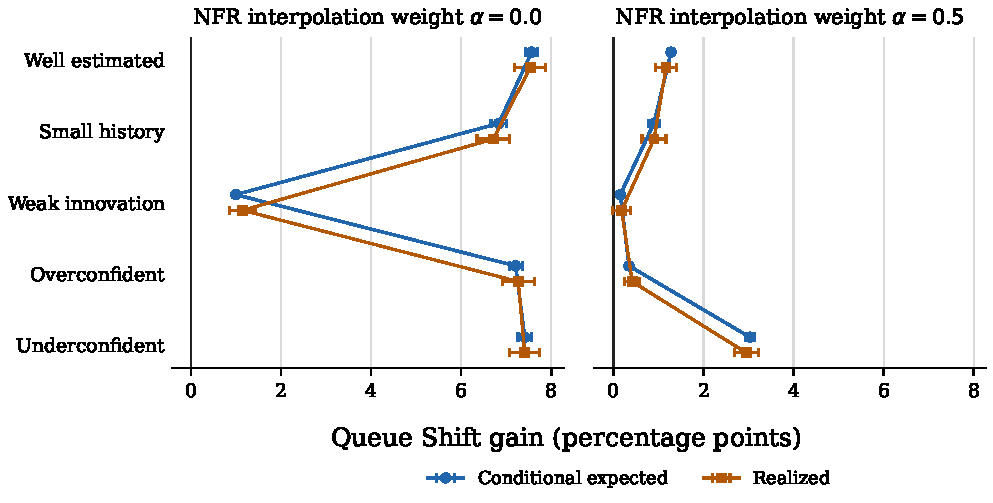
\includegraphics[width=0.96\linewidth]{figures/estimated_validation.pdf}
  \caption{Queue Shift gain over NFR interpolation at matched queue movement. Points are means
  across independently trained, accepted model updates; bars are 95\% normal intervals. Conditional
  expected accuracy uses the simulation's true probabilities and is not observable in deployment.}
  \label{fig:estimated-validation}
\end{figure}

The stress test also shows the limit of the claim. Under weak innovation at $\alpha=0.75$, the
mean conditional expected gain is approximately zero and slightly negative before rounding. At
$\alpha=1$, all scenarios satisfy the required score and accuracy equality. These results are
consistent with Equation~\ref{eq:error-bound}: optimizing noisy probabilities can lose a small
amount of true value when the available score advantage is nearly exhausted.

\section{What a deployment would validate}

A practical rollout separates model release from batch assignment. First, compare the raw
candidate with the incumbent on later labeled data and reject candidates that do not improve the
chosen predictive criterion. Second, choose an operational queue-shift budget. An existing NFR
rule can supply that budget, or managers can state it directly. Third, solve
Equation~\ref{eq:assignment} on each planning batch using candidate probabilities. Finally, monitor
queue loads by construction and evaluate accuracy when labels arrive.

The mathematical guarantee needs no labels at assignment time, but the expected-accuracy
interpretation needs useful probability scores. Reliability plots, proper scoring rules, and
out-of-time replay can diagnose that condition. Equation~\ref{eq:error-bound} also suggests a
direct sensitivity analysis: perturb candidate scores within an empirically plausible error set
and report how often the chosen assignment changes or loses value.

Three limitations matter before public claims become broad. First, the experiments assume a stable
population. They test a model innovation, not demand drift. Second, queue shift measures net load
redistribution, not the identities of workers or cases. Third, the evidence is synthetic. A field
study should report service times, queue-specific capacity, forecast horizon, and realized
staffing actions. Until then, the supported claim is the optimization guarantee and a simulation
showing that estimated scores can retain an advantage over the NFR-interpolation baseline.

\section{Conclusion}

For routing classifiers, compatibility is partly an allocation problem. NFR can remain valuable
for protecting individual decisions, but it cannot substitute for a measure of queue totals.
Queue Shift makes the operational constraint explicit and optimizes within it. The method weakly
dominates any comparison assignment under the common candidate score at the same queue movement,
and probability error determines whether that advantage transfers to true accuracy. This result
is modest, exact, and testable. It is a better foundation for deployment than treating a simulated
headline magnitude as a fact.

\appendix
\section{Oracle-posterior experiment}

As a mechanical check, an oracle experiment supplies the exact incumbent and candidate posteriors
from the same stable Gaussian population. The candidate observes an additional independent signal
and is released after an independent accuracy win. Figure~\ref{fig:oracle} shows the full matched
movement path. At the zero-movement endpoint, Queue Shift gains \ZeroMoveGain{} percentage points;
at the raw candidate endpoint, the gain is zero. These magnitudes describe this data-generating
process only.

\begin{figure}[H]
  \centering
  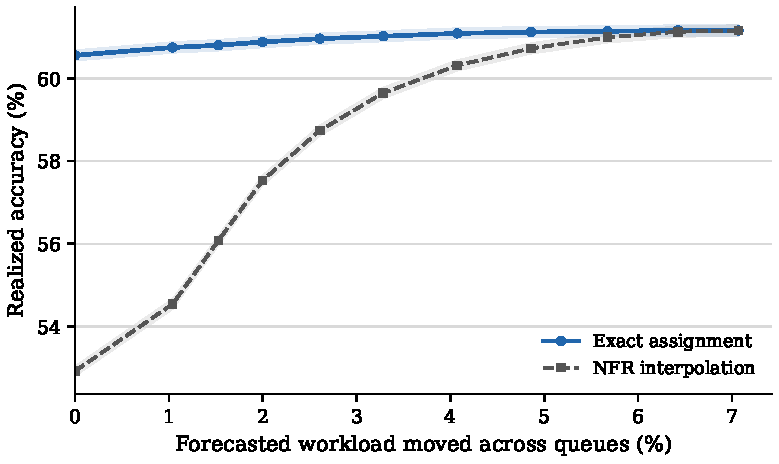
\includegraphics[width=0.82\linewidth]{figures/oracle_frontier.pdf}
  \caption{Oracle-posterior comparison at matched queue movement. Bands are 95\% normal intervals
  across independently generated updates.}
  \label{fig:oracle}
\end{figure}

\begin{table}[H]
\centering
\caption{Estimated-model validation against NFR interpolation}
\label{tab:estimated-validation}
\scriptsize
\begin{tabular}{lrrrrr}
\toprule
Scenario & $\alpha$ & Shift (\%) & Score gain & True gain [95\% CI] & Realized gain [95\% CI] \\
 & & & (pp) & (pp) & (pp) \\
\midrule
Well estimated & 0.0 & 0.00 & 7.75 & 7.56 [7.43, 7.70] & 7.54 [7.19, 7.88] \\
Well estimated & 0.5 & 3.82 & 1.35 & 1.28 [1.23, 1.33] & 1.17 [0.93, 1.41] \\
Well estimated & 1.0 & 7.42 & 0.00 & 0.00 [0.00, 0.00] & 0.00 [0.00, 0.00] \\
Small history & 0.0 & 0.00 & 8.53 & 6.84 [6.66, 7.01] & 6.71 [6.35, 7.08] \\
Small history & 0.5 & 4.11 & 1.48 & 0.90 [0.78, 1.02] & 0.90 [0.64, 1.17] \\
Small history & 1.0 & 7.88 & 0.00 & 0.00 [0.00, 0.00] & 0.00 [0.00, 0.00] \\
Weak innovation & 0.0 & 0.00 & 1.40 & 1.00 [0.96, 1.04] & 1.15 [0.86, 1.44] \\
Weak innovation & 0.5 & 1.89 & 0.33 & 0.15 [0.13, 0.18] & 0.18 [-0.02, 0.39] \\
Weak innovation & 1.0 & 3.02 & 0.00 & 0.00 [0.00, 0.00] & 0.00 [0.00, 0.00] \\
Overconfident & 0.0 & 0.00 & 13.30 & 7.21 [7.07, 7.35] & 7.27 [6.91, 7.62] \\
Overconfident & 0.5 & 5.42 & 0.91 & 0.35 [0.31, 0.38] & 0.42 [0.25, 0.59] \\
Overconfident & 1.0 & 7.57 & 0.00 & 0.00 [0.00, 0.00] & 0.00 [0.00, 0.00] \\
Underconfident & 0.0 & 0.00 & 3.60 & 7.41 [7.26, 7.56] & 7.41 [7.07, 7.75] \\
Underconfident & 0.5 & 2.76 & 1.42 & 3.03 [2.93, 3.13] & 2.95 [2.68, 3.22] \\
Underconfident & 1.0 & 7.45 & 0.00 & 0.00 [0.00, 0.00] & 0.00 [0.00, 0.00] \\
\bottomrule
\end{tabular}
\begin{minipage}{0.96\linewidth}
\footnotesize\emph{Note:} Multinomial logistic models are estimated on historical samples and released only after the candidate wins on an independent labeled sample. Each row compares exact assignment with probability interpolation at the same realized queue shift. True gain uses the simulation's conditional probabilities and is unavailable in applications. Results average four planning batches within each independently trained accepted update before averaging across updates.
\end{minipage}
\end{table}

\begin{table}[H]
\centering
\caption{NFR interpolation versus exact assignment at the same queue shift}
\label{tab:stable-update}
\small
\begin{tabular}{rrrrrr}
\toprule
Interpolation & Queue shift & NFR & NFR path & Exact assignment & Gain \\
$\alpha$ & (\%) & (\%) & accuracy (\%) & accuracy (\%) & (pp) \\
\midrule
0.0 & 0.00 & 0.00 & 52.92 & 60.56 & 7.64 \\
0.2 & 1.53 & 2.30 & 56.08 & 60.80 & 4.72 \\
0.5 & 3.28 & 6.49 & 59.65 & 61.02 & 1.37 \\
0.8 & 5.67 & 10.79 & 60.99 & 61.14 & 0.15 \\
1.0 & 7.07 & 13.28 & 61.16 & 61.16 & 0.00 \\
\bottomrule
\end{tabular}
\begin{minipage}{0.94\linewidth}
\footnotesize\emph{Note:} The data-generating process is fixed across release and planning samples. The candidate observes an additional independent signal and is deployed only after beating the incumbent on an independent out-of-sample release set. Each row compares probability interpolation with the exact assignment using the candidate posterior at the interpolation point's realized queue shift. Results average 1,000 planning batches from 200 accepted updates. Percentage-point gains use labels revealed only after both assignments are fixed.
\end{minipage}
\end{table}


\bibliographystyle{apalike}
\bibliography{references}

\end{document}
